\clearpage
\chapter{EXTRACTION OF BRUSH STROKES}

Brush strokes normally follow certain rules in a brush painting and they vary depending the type of paintings. Here we discuss how we make use of such rules. Rosemaling paintings usually use subtle and vibrant colors to enhance color contrast between overlapped strokes. As a result, the overlapped strokes tend to be classified into different layers. Extracting brush strokes within one layer is easier than directly from the input painting. We employ the Maximally Stable Extremal Regions (MSERs) proposed in \cite{donoser2006efficient} and \cite{nister2008linear} to extract brush strokes since it is invariant to affine intensity changes. MSERs algorithm requires a distinct difference between background and foreground while allowing a small variation of intensity within the selected stroke region. Usually, the strokes on the decomposed layers satisfy this requirement.


However, it is likely that MSERs may fail in segmentation with the following scenarios,\newline (1) two adjacent regions with the similar intensity; \newline (2) the region with a high transparency. \newline
(3) Moreover, like the other existing segmentation approaches, the MSERs algorithm encounters over-segmentation issue as well. To tackle these challenges, the coherent lines \cite{kang2007coherent} is introduced into MSERs, which both enhances the edges of strokes and preserves the completeness of strokes. For completeness sake, we briefly address MSERs algorithm and then address our modification.
\section{MSERs Algorithm}
Maximally Stable Extremal Regions (MSERs) \cite{matas2004robust} can denote a set of distinguished regions that are detected in a gray scale image. All of these regions are defined by an extremal property of the intensity function in the region and on its outer boundary. MSERs have properties that form their superior performance as stable local detector. The set of MSERs is closed under continuous geometric transformations and is invariant to affine intensity changes. Furthermore MSERs are detected at different scales.

MSER requires a data structure that can be efficiently built and managed. The component tree is a structure which allows the detection of MSERs within an image and, in addition, constitutes the basis for MSER tracking. The component tree has been recently used for efficient implementation of watershed segmentation \cite{couprie2005algorithms} .
\begin{figure}[H]
	\centering 
	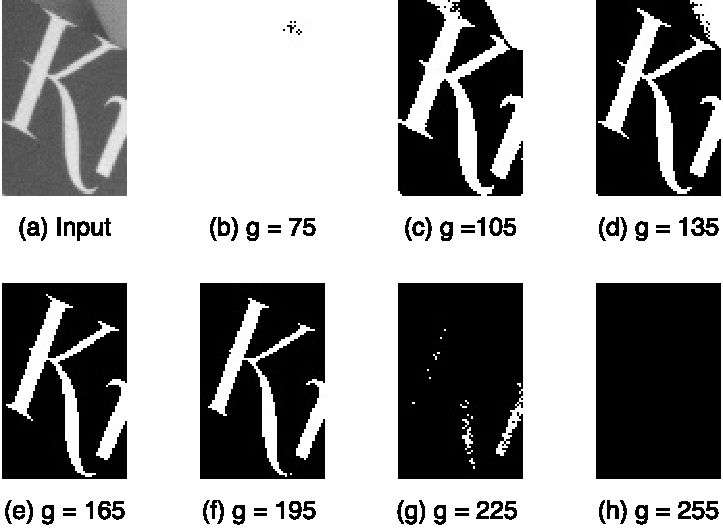
\includegraphics[width=10cm]{mser_threshold.pdf}
	\caption{Extreme regions based on threshold}
	\label{mser:K}
	\medskip
	\small	
	Threshold images analyzed during creation of component tree. Figure (a) shows the considered area and figures (b) to (g) the results of thresholding this image at gray level g. The letter k is identified as MSER because the size of the connected region does not change significantly in the gray level range from 135 to 195.
	
\end{figure}
 
The edges within the tree define an inclusion relationship between the connected regions. Thus, for a region  that is the son of another region  within the tree,
is fulfilled. By moving in the component tree upwards, the corresponding intensity value $g$ of the extremal regions becomes lower, which leads to increased region sizes. The root of the tree represents a region which includes all pixels of the input image . Figure \ref{mser:tree} shows typical parts of the component tree created for the image shown in Figure \ref{mser:K}(a).


MSERs can denote a set of distinguished regions that are detected in an intensity image. All of these regions are defined by an extremal property of the intensity function in the region and on its outer boundary, i.e. for a given extremal region S, the internal intensity is more than the intensity of boundary of S,

\[ \forall p \in S,\forall q \in \partial S , \longrightarrow I(p) \geq I(q)\]

where $\partial S $ denotes the boundary of $S$.
Changing threshold, the extremal regions may further split or merge. The resulting extremal regions may be represented by the component tree. Accordingly, we may compute the change rate of the area of extremal region by,
\begin{figure}[H]
	\centering 
	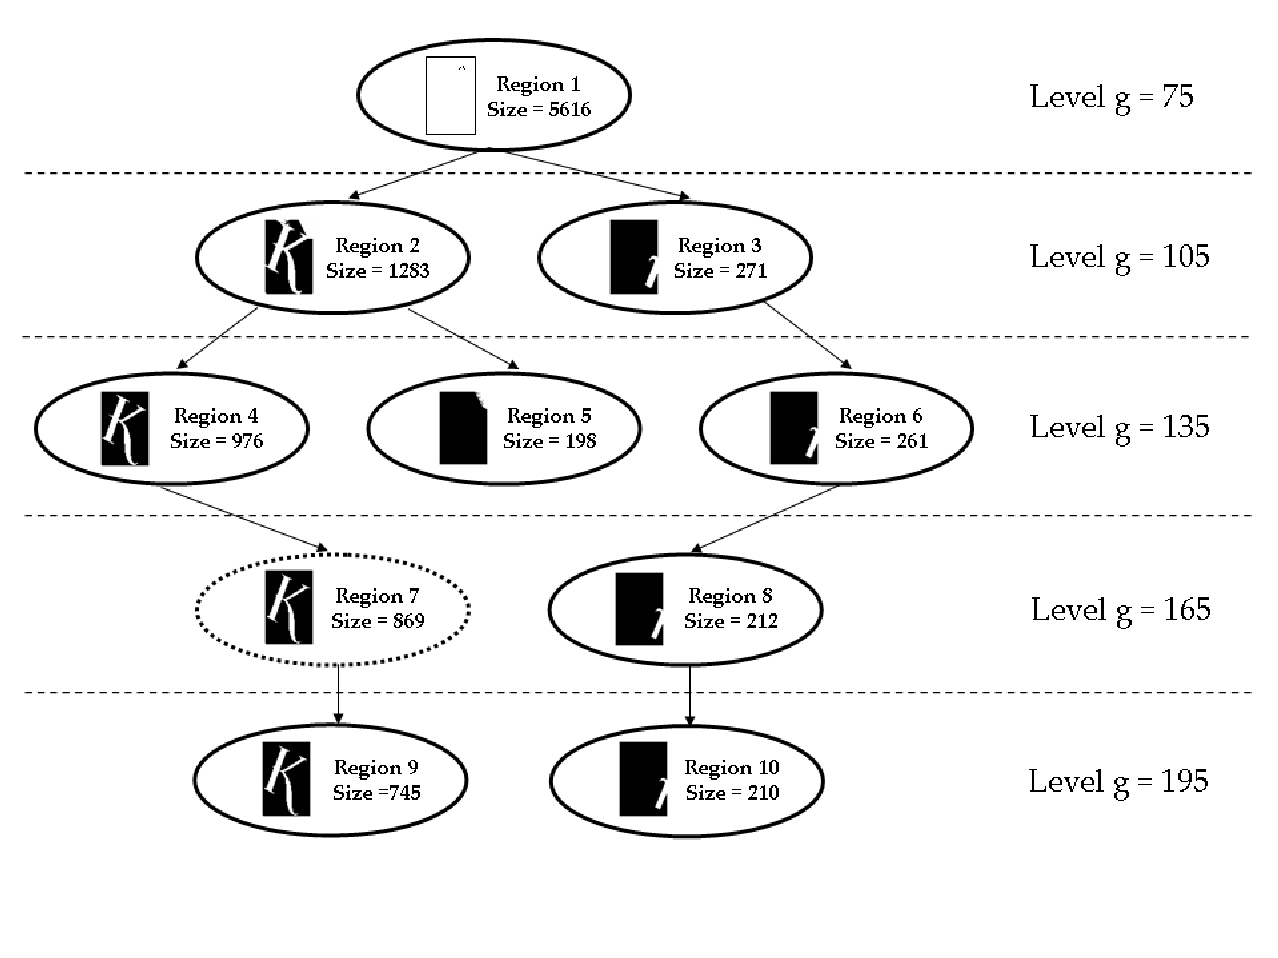
\includegraphics[width=13cm]{MSER_tree.png}
	\caption{MSER tree}
	\label{mser:tree}
	\medskip
	\small
	Parts of the created component tree for the input image. Region 7 is identified as MSER.
\end{figure}


\[ \gamma(S_i^g) = \frac{\left ( \left |  S_j^{g-\Delta} \right |-\left |  S_k^{g+\Delta} \right | \right )}{\arrowvert S_i^g\arrowvert} \]

where $ \left | .  \right |$  denotes the cardinality, $ S_{i}^{g} $  is the i-th region which is obtained by thresholding at an intensity value g and $\Delta $ is a stability range parameter. $  g-\Delta $ and $ g+\Delta $ are obtained by moving upward and downward respectively in the component tree from the region $ S_{i} $ until a region with intensity value   or  is found. $ \left \{ i,j,k \right \}$ are the indices of nodes of the component tree. MSERs correspond to those nodes of the component tree that have a stability value $\gamma$, which is a local minimum along the path to the root of the tree.

\begin{figure}[H]
	\centering 
	
\includegraphics[width=8cm]{inten_mser.png}
	\caption{  MSERs on the intensity of image}
	\medskip
	\small
	Perform the original MSERs on the intensity of image; It is clear to see over-segmentation.
\end{figure}

\section{Modified MSERs Algorithm}
\begin{figure}[H]
	\centering 
	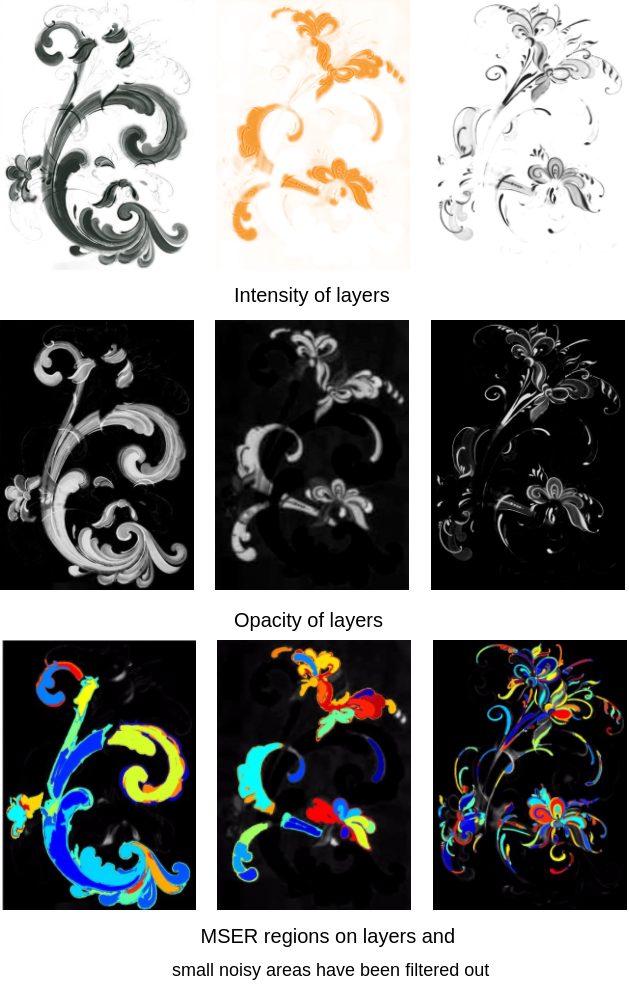
\includegraphics[width=10cm]{layer_sum.png}
	\caption{The intensity, opacity maps, and MSER regions of three layers by the modified MSERs.}
	\label{mser:alpha}
\end{figure}
In terms of the definition of the area change rate $\gamma$, MSERs may fail in segmentation with the following scenarios,\newline (1) the region with the intensity very close to the background; \newline (2) two adjacent regions with the similar intensity; \newline (3) the region with a very high transparency. \newline The opacity of the image, $\alpha$, is always independent of the intensity of the image. It is likely to avoid the abovementioned scenarios if segmentation can be performed on $\gamma$. We perform the layer decomposition of Eq \ref{eq:layer_sum} on a brush painting and show the intensity and opacity of one layer associated with the individual histograms in Figure \ref{histo}. It can be noted that the opacity of the layer contains richer layered details than the intensity. Moreover, Table 1 also shows that the opacity of the layers is more suitable for stroke segmentation than the intensity. The first modification is to perform MSERs on the opacity of every layer.
We aim at the scenarios of two adjacent regions with the similar opacity. When the extremal region is growing up through changing threshold, it is feasible to restrict the region by introducing the coherent lines. According to the definition of the extremal region, the boundary of region S should satisfy,

\begin{equation*}
 \forall p \in S,\forall z \in   \bar{S} , \forall q \in \partial S \longrightarrow I(p) \geq I(q)  ~\mathrm{and}~  I(q) \leq I(z)
\end{equation*}
 
where $ \bar{S} $ denotes the complement of $S$. The second modification is to simply modify the opacity of layers, that is, overlapping the coherent lines with the layer and then changing the opacity of coherent lines to the smallest value in the layer.

To deal with the over-segmentation issue, the coherent lines play an important role. Given a region $S$, we modify the area change rate $\gamma$ as,
\begin{equation}
\gamma(S_i^g)=\frac{  \lvert \lvert S_j^{g-\Delta}\rvert -\lvert S_k^{g+\Delta} \rvert
	 \rvert     }{\arrowvert S_i^g\arrowvert} + \frac{  \lvert \lvert Q_j^{g-\Delta}\rvert -\lvert Q_k^{g+\Delta} \rvert
	 \rvert     }{\arrowvert Q_i^g\arrowvert} - (1-\frac{\lvert Q_i\rvert}{\lvert \partial S_i^g \rvert} )
\end{equation}


where $Q$ denotes the set of pixels which stay on the coherent lines and $Q \subset \partial S $. The third modification is to take into account the change of coherent lines to the boundary of $S$, i.e. the third term penalizes that a small portion of the boundary $\partial S$ is occupied by coherent lines.

Figure \ref{mser:alpha} shows the segmentation results by the modified MSERs, which correspond to brush strokes. It can be noted that performing MSERs on the intensity of image inevitable yields over-segmentations. Performing the modified MSERs on the opacity of layers, the strokes tend to complete and smooth within one layer. Moreover, some small regions with the distinct opacity values against neighboring areas have been filtered out.
 


\begin{figure}[H]
	\centering
	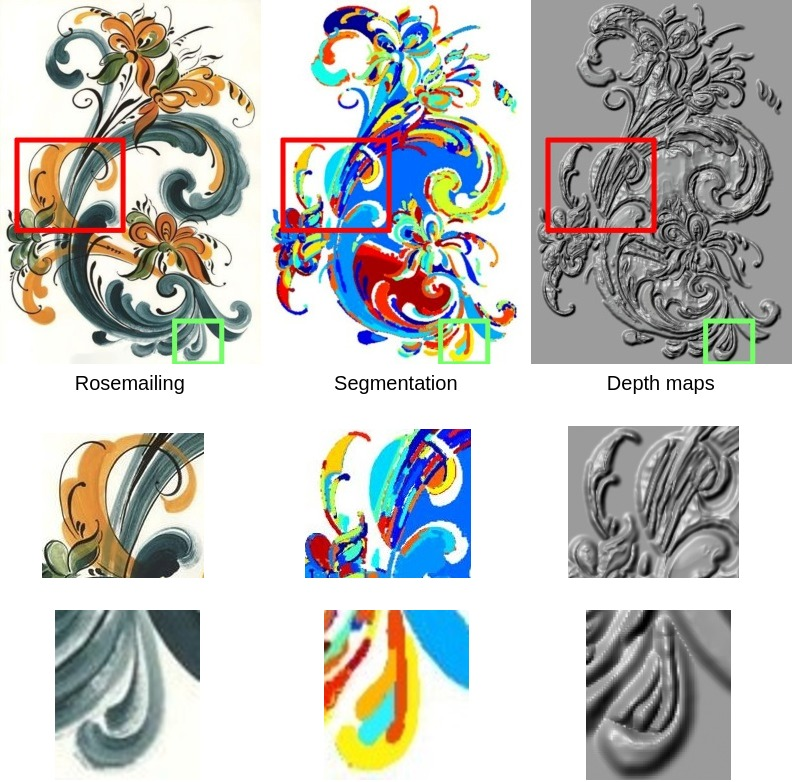
\includegraphics[width=15cm]{overseg.jpg}
	\caption{Incorrect and over segmentation}
	\label{overseg}
	\medskip
	Resulting depth maps based on segmentation of image intensity. Second row shows the incorrect segmentation (brown area in Top is missed in Middle);Last shows the over-segmentation (2 patches in Top are divided into 4 parts in Middle).
\end{figure}






